Автокорреляция — это метод оценки зависимости значений последовательности от её предыдущих значений. Лаг \( k \) показывает, насколько текущие значения последовательности \( x_t \) зависят от значений \( x_{t-k} \), стоящих на \( k \) позиций ранее. Формула расчёта коэффициента автокорреляции на лаге \( k \):

\[
	r_k = \frac{\sum_{t=k+1}^{T} (x_t - \bar{x}) (x_{t-k} - \bar{x})}{\sum_{t=1}^{T} (x_t - \bar{x})^2}
\]

Здесь \( \bar{x} \) — среднее значение последовательности, а \( T \) — общее количество элементов. Автокорреляционный анализ выявляет закономерности в данных: высокий коэффициент указывает на зависимость между текущими и предыдущими значениями.
\subsection{Выполнение автокорреляционного анализа}

В таблице ниже представлены коэффициенты автокорреляции для различных сдвигов (от 1 до 10) как для исходной последовательности, так и для сгенерированной числовой последовательности. Количество элементов последовательности \( T = 300 \).

\begin{table}[H]
	\centering
	\resizebox{\textwidth}{!}{
		\begin{tabular}{|c|c|c|c|c|c|c|c|c|c|c|}
			\hline
			\textbf{Сдвиг ЧП}                     & \textbf{1} & \textbf{2} & \textbf{3} & \textbf{4} & \textbf{5} & \textbf{6} & \textbf{7} & \textbf{8} & \textbf{9} & \textbf{10} \\
			\hline
			\textbf{К-т АК} для зад. \textbf{ЧП}  & -0.0206    & -0.0099    & 0.0579     & 0.0680     & -0.0160    & -0.0047    & 0.0170     & -0.0307    & -0.0334    & 0.0260      \\
			\hline
			\textbf{К-т АК} для сген. \textbf{ЧП} & -0.0464    & 0.0167     & 0.0242     & -0.0350    & 0.0909     & -0.0560    & -0.0495    & -0.0452    & -0.0632    & -0.0089     \\
			\hline
			\textbf{\% откл.}                     & 125.243    & -268.687   & -58.204    & -151.471   & -668.125   & 1091.49    & -391.176   & 47.231     & 89.222     & -65.769     \\
			\hline
		\end{tabular}
	}
	\caption{Коэф. автокорреляции для заданной и сгенерированной ЧП}
\end{table}

\subsection{Результаты автокорреляционного анализа}

Для оценки случайности последовательности использовалось пороговое значение коэффициента автокорреляции — 0.2. Если автокорреляция на сдвиге превышает это значение, последовательность можно считать неслучайной. Но как видно из талицы и графика, ни одно из значений коэффициентов корелляции для исходной последовательности не превышает даже 0,1 -- исходя из этого можно сделать вывод, что числовая последовательность является случайной.

\begin{figure}[H]
	\centering
	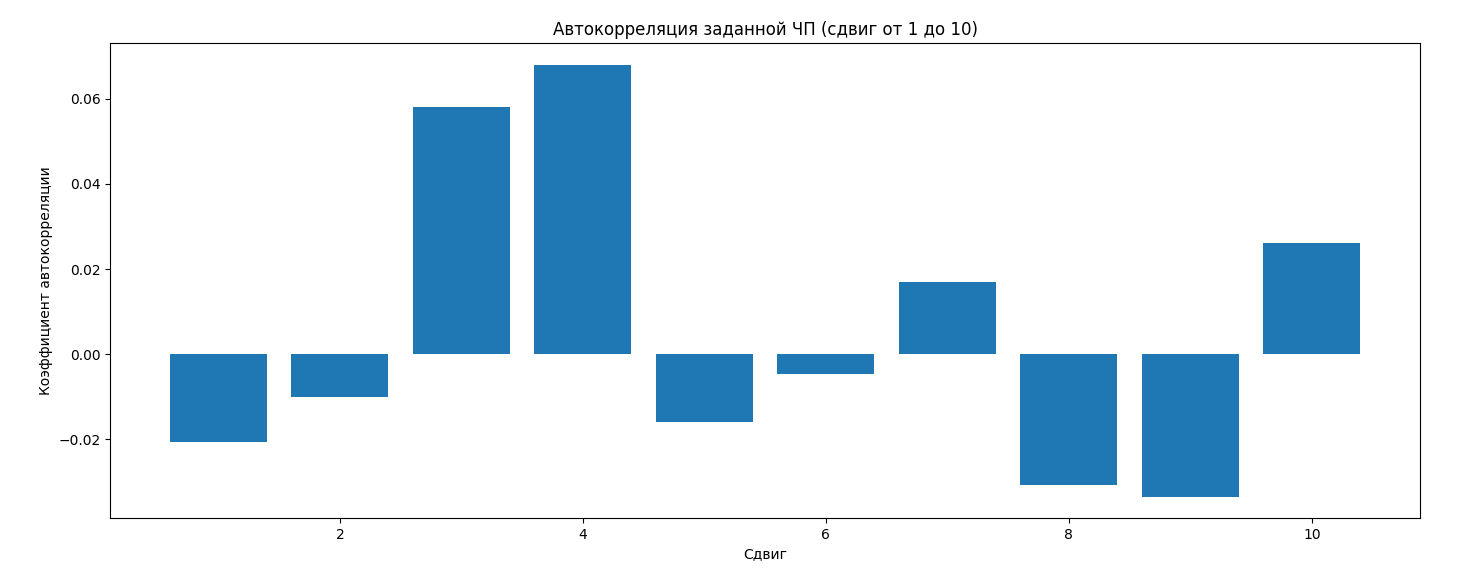
\includegraphics[width=1\textwidth]{../data/auto_corellation-1.png}
	\caption{Автокорреляционный анализ для заданной ЧП}
\end{figure}


\subsection{Анализ сгенерированной последовательности}

\begin{figure}[H]
	\centering
	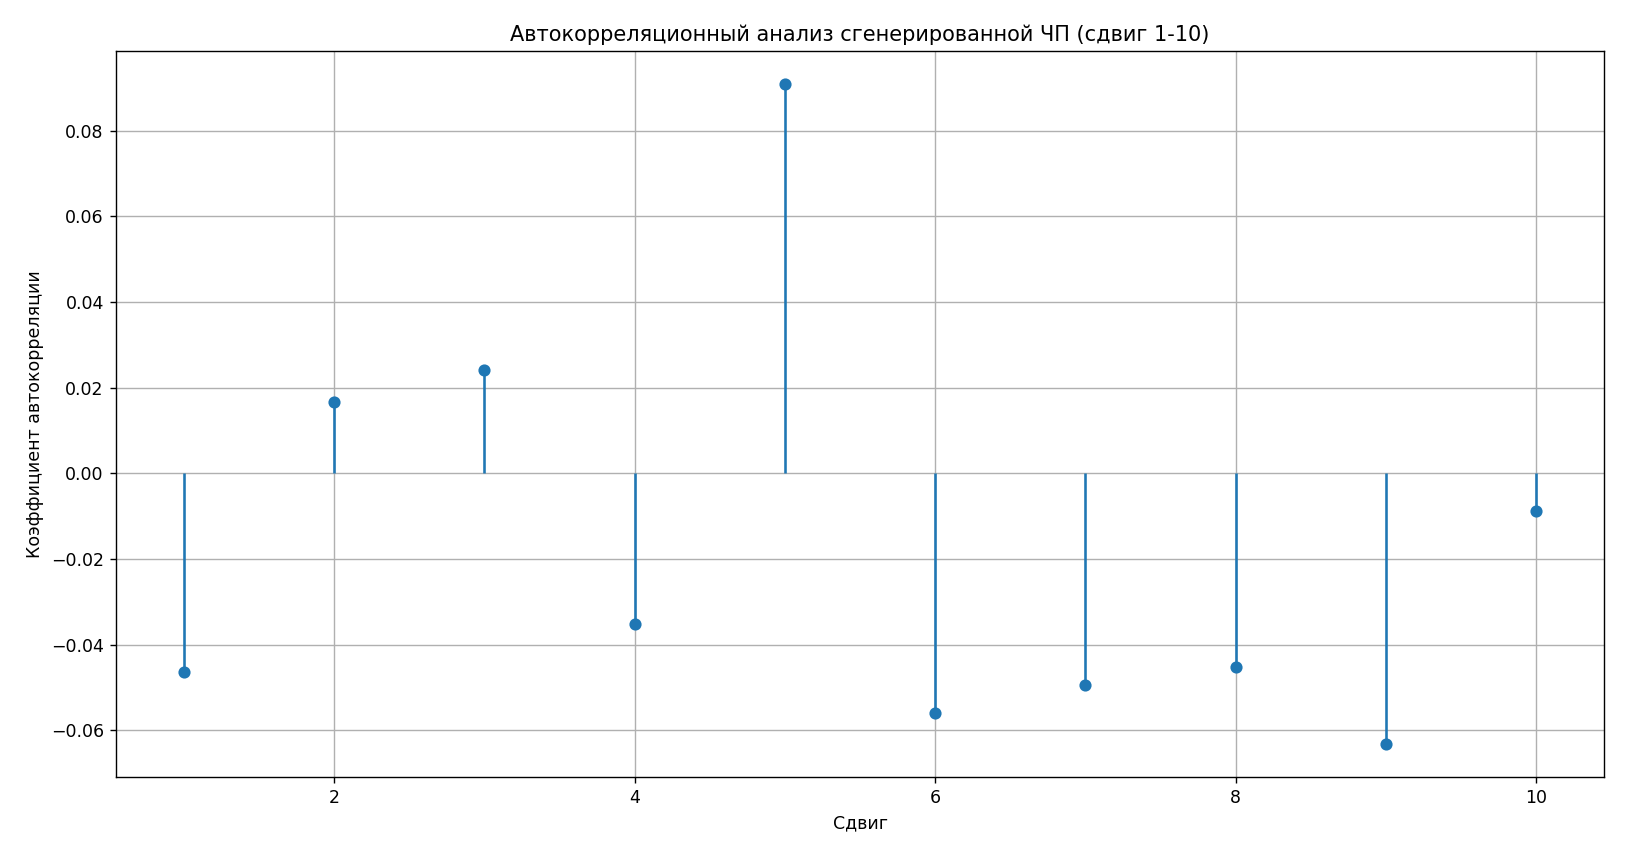
\includegraphics[width=1\textwidth]{../data/auto_corellation-2.png}
	\caption{Автокорреляционный анализ для сгенерированной числовой последовательности}
\end{figure}

Аналогичный анализ был проведён для сгенерированной числовой последовательности. Как показано на графике и в таблице, все коэффициенты автокорреляции для сгенерированной последовательности также не превышают порога 0.1, что позволяет заключить, что сгенерированная последовательность является случайной.

\subsection{Выводы}

На основании автокорреляционного анализа можно сделать следующие выводы:
\begin{itemize}
	\item Заданная числовая последовательность не имеет значимых зависимостей между значениями на различных сдвигах. Все коэффициенты автокорреляции для сдвигов от 1 до 10 не превышают порога 0.1, что позволяет считать последовательность \textbf{хаотичной}.
	\item Сгенерированная числовая последовательность также демонстрирует случайный характер, так как коэффициенты автокорреляции не превышают значения 0.1.
\end{itemize}
